\documentclass[conference]{IEEEtran}

\usepackage{amsmath}
\usepackage{amssymb}
\usepackage{booktabs}
\usepackage{array}
\usepackage{graphicx}
\usepackage{multirow}
\usepackage{tikz}
\usepackage{url}
\usepackage{cite}
\usepackage{xcolor}
\usepackage{listings}
\usepackage[hidelinks]{hyperref}
\usetikzlibrary{arrows.meta,positioning}

\newcommand{\system}{AuthGuard-7702}
\newcommand{\model}{AuthGuard-Seq}
\newcommand{\bench}{AuthGuardBench-7702}
\newcommand{\bclear}{\texttt{benign\_cleared}}
\newcommand{\bgen}{\texttt{benign\_general}}
\newcommand{\baa}{\texttt{benign\_AA}}
\newcommand{\code}[1]{\texttt{#1}}

\lstset{
  basicstyle=\ttfamily\scriptsize,
  frame=single,
  breaklines=true,
  columns=fullflexible,
  showstringspaces=false,
  xleftmargin=2pt,
  xrightmargin=2pt
}

\begin{document}

\title{AuthGuard-7702: Hierarchical Bytecode Sequence Screening for EIP-7702 Delegation}

\author{\IEEEauthorblockN{Anonymous Authors}}

\maketitle

\begin{abstract}
EIP-7702 allows an externally owned account to delegate execution to contract code, creating a
security-critical decision before the account signs an authorization. At that point, a malicious
delegate may have no transaction history, reputation, or verified source code, limiting
behavior-dependent defenses. We present \system, an integration-ready, bytecode-only screening
tool that analyzes delegate runtime code before authorization and returns a risk score,
policy-derived warning level, directly observed security indicators, and structured output. Its
core, \model, is a lightweight hierarchical opcode-sequence model that encodes local instruction
patterns in 256-token chunks and aggregates contract-wide evidence through learned attention. We
evaluate the system on \bench, a task-aligned corpus with 2,280 primary contracts from 819
bytecode families, 797 additional benign controls, exact-duplicate controls, and bounded bytecode
transformations. Across three training seeds, \model{} achieves mean family-disjoint AUPRCs of
0.931 on clean bytecode, 0.910 under 200\% donor-isolated flooding, and 0.910 under combined
selector/address rewriting and flooding, compared with 0.828, 0.577, and 0.563 for the strongest
histogram+n-gram XGBoost baseline. In a primary-seed paired family-clustered analysis, clean AUPRC
improves by 0.057 (95\% CI 0.002--0.118), while recall at the 5\% false-positive policy improves
by 0.212. The 0.743 MB model completes local preprocessing, inference, policy evaluation, and
evidence generation in 4.334 ms on average (p95 14.073 ms) over 3,000 CPU calls. These results
establish the feasibility of lightweight pre-authorization delegate screening while exposing a
remaining benign-control false-alert tradeoff and clear limits on semantic and wallet-level
claims.
\end{abstract}

\begin{IEEEkeywords}
EIP-7702, account delegation, smart-contract security, bytecode sequence learning,
pre-authorization screening, adversarial evaluation
\end{IEEEkeywords}

\section{Introduction}
\label{sec:introduction}

EIP-7702 changes the security boundary of an externally owned account (EOA). An EOA may sign an
authorization that installs the designator $\mathtt{0xef0100}\,\|\,\mathit{address}$ in its code
field; subsequent calls load code from the referenced delegate while executing in the authority
account's context~\cite{eip7702}. This construction enables batching, sponsored execution, and
programmable account policies without migrating assets to a new account. It also makes delegate
selection consequential: code that is malicious, compromised, or overly permissive can exercise
authority associated with an established EOA~\cite{qi2025eip7702phishing,huang2026darkside}.

The defensive decision precedes the authorization signature. A new delegate can lack the
transaction history, victim reports, counterparty graph, and reputation signals used by many
phishing detectors. Verified source code may also be absent. Runtime bytecode at the proposed
delegate address is nevertheless observable and can be inspected locally. Existing EIP-7702 work
has already established malicious delegation and phishing risks using transaction analysis,
decompilation, and cross-contract static reasoning~\cite{qi2025eip7702phishing,huang2026darkside}.
Our question is narrower: can bytecode alone provide a useful, low-latency warning \emph{before}
the signer authorizes the delegate? To our knowledge, the literature does not yet establish an
EIP-7702-specific, ML-based, bytecode-only screener at this decision point. This wording does not
claim the first EIP-7702 detector or the first learned bytecode security analyzer.

This task presents several technical and methodological challenges. Exact deployments and
near-duplicate compiler variants violate the independence assumed by random splits. Long runtime
programs exceed the fixed prefixes used by ordinary sequence encoders. Metadata, embedded
addresses, selectors, and appended bytes can change surface representations without necessarily
removing the behavior of concern. Finally, a useful warning system must operate at explicit
false-positive budgets, expose the scope of its evidence, and avoid disguising local model timing
as end-to-end wallet latency.

We address these challenges with \system. The tool accepts raw runtime bytecode, a delegate
address with an RPC endpoint, or one EIP-7702 authorization entry. It normalizes and tokenizes the
delegate runtime, applies a hierarchical full-bytecode sequence model, temperature-scales the
score, maps it to thresholds fitted at nominal 1\%, 5\%, and 10\% validation-negative
false-positive rates (FPRs), and returns a structured warning with deterministic bytecode
observations. The selected model uses neither a decompiler nor transaction history, family,
address, chain, fold, or label-construction fields. It also does not truncate at the first linear
\code{STOP}: our audit found that post-\code{STOP} code was statically reachable in all 727
malicious samples, making first-\code{STOP} a predictive but non-semantic shortcut.

We evaluate \system{} on \bench. The primary task comprises 727 artifact-derived malicious
delegates and 1,553 rule-silent weak negatives, arranged into 819 frozen bytecode families. The
benchmark retains 797 broader benign controls, constrains exact duplicates to one label and fold,
and evaluates clean, F200, and M3+F200 conditions. At the three-seed level, \model{} reaches 0.931
clean AUPRC versus 0.828 for histogram+hashed-4-gram XGBoost. Under F200 and M3+F200, it maintains
approximately 0.910 AUPRC, while the baseline falls to 0.577 and 0.563. The primary paired
analysis confirms positive clean and transformed AUPRC and Recall@5 gains, but the independent
benign-control comparison does not support a lower false-alert claim. This distinction is central
to our deployment interpretation.

The paper makes three contributions:
\begin{itemize}
  \item \textbf{Operational pre-authorization screening.} We introduce \system, an
  integration-ready CLI/Python tool that accepts bytecode, addresses, or authorization entries
  and emits a calibrated risk score, validation-derived warning level, directly observed opcode
  evidence, model provenance, and JSON output.
  \item \textbf{Hierarchical opcode-sequence learning.} We design \model, a compact architecture
  that preserves contract-wide coverage through chunk encoding and learned attention. It
  significantly improves clean and bounded-transformation detection over the strongest evaluated
  bytecode baseline under family-disjoint evaluation.
  \item \textbf{Dependence-aware benchmark and operational evaluation.} We provide \bench{} and
  an evaluation protocol combining task alignment, frozen family and duplicate controls, benign
  controls, matched-FPR policies, donor-isolated transformations, paired family-clustered
  uncertainty, per-row artifacts, and local runtime measurement.
\end{itemize}

\section{Background and Related Work}
\label{sec:related}

\subsection{EIP-7702 delegation and authorization risk}

An authorization tuple identifies a delegate address. Processing the tuple places a 23-byte
delegation designator at the authority account; it does not copy the referenced runtime program
into that field~\cite{eip7702}. A bytecode screener must therefore resolve the delegate and inspect
its runtime rather than classify the authority's designator. Execution retains the authority
account's context, so delegate logic can interact with its storage, balances, and permissions.
The EIP's own security considerations require signers to trust delegated code and account for
authorization replay and initialization behavior~\cite{eip7702}.

Recent studies demonstrate that this trust can be abused. Qi et al. describe phishing workflows
involving user- and attacker-driven authorization activation and cross-chain concerns
~\cite{qi2025eip7702phishing}. Huang et al. develop a taxonomy of EOA-targeted,
contract-targeted, and composite risks and analyze observed delegates with transaction and
cross-contract methods~\cite{huang2026darkside}. These analyses motivate the task and provide a
source for the positive observations used here. They are complementary to our decision point:
\system{} is an early screening layer, not a reproduction or replacement of full cross-contract
analysis.

\subsection{Learning-based Ethereum security}

Ethereum phishing detection has been studied using transaction payloads, temporal account
features, and graph structure~\cite{chen2025ptxphish,chen2020ijcai,chen2020toit}. Such context is
valuable after activity exists but may be unavailable for an unused delegate. Code-based systems
instead derive signal from program artifacts. PhishingHook compares EVM opcode and bytecode
representations for phishing-contract classification~\cite{derosa2025phishinghook}; ContractWard
uses opcode bigrams for vulnerability classification~\cite{wang2021contractward}. These studies
support the premise that bytecode contains learnable security signal, but their labels and
operating decisions differ from EIP-7702 authorization. We therefore do not compare published
metrics across datasets. Representative bytecode representations are retrained on the same
\bench{} folds.

\subsection{Static analysis, dependence, and adversarial representation}

Static analyzers recover richer semantics than a lightweight scorer. Gigahorse constructs an EVM
intermediate representation for declarative analysis~\cite{grech2019gigahorse}; Securify derives
program dependencies and checks compliance and violation patterns~\cite{tsankov2018securify}.
These tools can be used after a fast model warning or in high-value cases. We do not benchmark
them and make no relative speed or detection claim.

Security evaluation is easily inflated when related artifacts cross partitions. TESSERACT shows
how spatial and temporal biases distort malware-classifier estimates~\cite{pendlebury2019tesseract},
while Transcend addresses concept drift in deployed classifiers~\cite{jordaney2017transcend}.
We apply the former principle by preserving bytecode-similarity families and grouping exact
duplicates. This controls a known dependence source but does not substitute for future temporal
or cross-ecosystem validation.

Executable-domain attacks must also be assessed in the problem space. Prior malware work studies
constrained adversarial examples and the gap between feature-space and realizable
transformations~\cite{grosse2017adversarial,pierazzi2020problemspace}. Our stress tests similarly
modify actual byte strings, but the guarantee is narrower: they are bounded, protocol-defined
transformations with donor isolation and limited execution checks. They do not establish
universal semantic equivalence or robustness to arbitrary recompilation.

\section{Problem Definition and Threat Model}
\label{sec:problem}

\subsection{Pre-authorization risk screening}

Let $b\in\mathcal{B}$ be normalized runtime bytecode at the delegate address and let $T(b)$ be its
deterministic opcode-token sequence. A trained model $f_\theta$ produces a logit $z$, which is
temperature-scaled on held-out validation data:
\begin{equation}
  s(b)=\sigma\!\left(\frac{f_\theta(T(b))}{\mathcal{T}}\right), \qquad s(b)\in[0,1].
  \label{eq:score}
\end{equation}
The score ranks evidence associated with the benchmark's delegate-risk label. It is not a
probability of asset theft and does not certify safety.

Let $\tau_{1}\geq\tau_{5}\geq\tau_{10}$ be thresholds estimated only from negative validation
scores at nominal 1\%, 5\%, and 10\% FPR. The external warning policy is
\begin{equation}
  \pi(s)=
  \begin{cases}
    \textsc{high}, & s\geq\tau_1,\\
    \textsc{warning}, & \tau_5\leq s<\tau_1,\\
    \textsc{caution}, & \tau_{10}\leq s<\tau_5,\\
    \textsc{low-observed-risk}, & s<\tau_{10}.
  \end{cases}
  \label{eq:policy}
\end{equation}
Because finite held-out samples and distribution shift can change achieved FPR, the nominal policy
name and observed test FPR are reported separately.

\subsection{Information available to the defender}

The defender supplies runtime bytecode directly or supplies an address/authorization from which
the integration fetches bytecode. The model may observe opcode order and bytecode-local
immediates exposed by tokenization. It does not receive past or future transactions, signer
balances and approvals, counterparties, verified source, decompiler facts, chain identity,
contract address, family/fold identifiers, or fields used to construct the source labels. The
tool's evidence extractor separately reports static occurrences of call-family, storage,
delegation, token-selector, approval-selector, and code-lifecycle surfaces. These observations do
not establish control-flow reachability, intent, or exploitability.

\subsection{Adversary and excluded claims}

The evaluated adversary may rewrite a recognized metadata trailer, selected \code{PUSH20} address
immediates, and sensitive \code{PUSH4} selectors; it may also append partition-isolated donor
bytes after \code{STOP}. F200 appends bytes equal to 200\% of the source executable length.
M3+F200 composes metadata, address, and selector rewriting with the 200\% flood. Donors are drawn
from benign-general sources isolated by outer fold and partition.

This adversary does not cover arbitrary recompilation, control-flow obfuscation, dynamic code
generation, changed proxy state, new malicious semantics absent from the labels, or white-box
optimization against the final model. Address and selector rewriting may change behavior. In a
bounded ten-contract, 100-call audit, F200 preserved the recorded execution fingerprint in
100/100 calls, whereas M3-related rewrites preserved it in only 23/100. Consequently, transformed
results are stress-test evidence, not a semantic-equivalence claim.

\subsection{Deployment boundary}

The implemented system includes parsing, local preprocessing, inference, policy evaluation,
direct-evidence extraction, and JSON-ready result construction. RPC correctness, delegation and
proxy-chain resolution, caching, wallet UI, user response, and transaction blocking are outside
the evaluated system. The output is advisory. Operational deployment should pair it with trusted
bytecode retrieval, clear residual-risk language, and escalation to deeper analysis where
appropriate.

\section{System Architecture}
\label{sec:system}

\subsection{End-to-end workflow}

Figure~\ref{fig:workflow} separates the implemented scoring path from optional integration
context and offline fitting. Three input modes share the same core:
\begin{enumerate}
  \item \code{scan-bytecode} scores a supplied runtime without network access;
  \item \code{scan-address} retrieves runtime using \code{eth\_getCode}; and
  \item \code{scan-authorization} extracts one delegate address from an authorization object and
  applies the address path.
\end{enumerate}
The scorer validates nonempty normalized bytecode, tokenizes it, applies the saved model and
temperature, maps the result through the saved warning policy, extracts direct evidence, and
returns a versioned result. The Python \code{AuthGuardScorer} provides the same functions without
subprocess or text parsing.

\begin{figure*}[t]
  \centering
  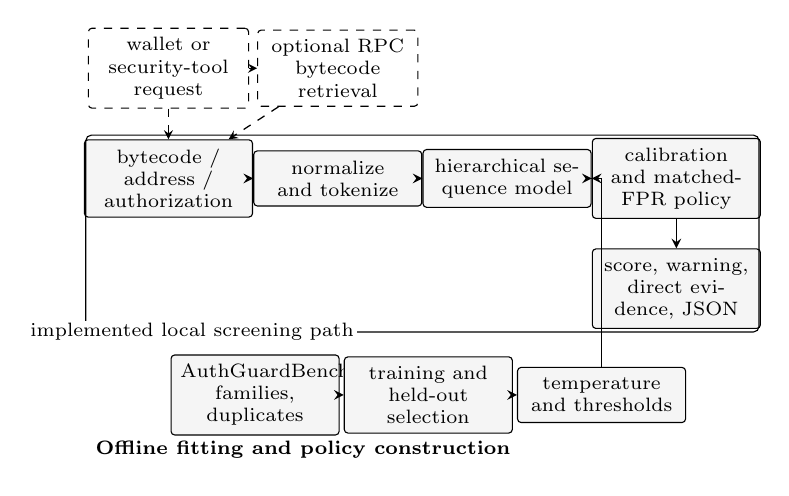
\begin{tikzpicture}[
  font=\scriptsize,
  box/.style={draw, rounded corners=1.3pt, minimum height=7mm, text width=19mm,
              align=center, fill=gray!8},
  ext/.style={draw, dashed, rounded corners=1.3pt, minimum height=7mm, text width=18mm,
              align=center},
  flow/.style={->, >=stealth, line width=.55pt},
  context/.style={->, >=stealth, dashed, line width=.45pt}
]
  \node[ext] (wallet) at (-3.2,2.0) {wallet or security-tool request};
  \node[ext] (rpc) at (-1.05,2.0) {optional RPC bytecode retrieval};
  \node[box] (input) at (-3.2,.6) {bytecode / address / authorization};
  \node[box] (token) at (-1.05,.6) {normalize and tokenize};
  \node[box] (model) at (1.10,.6) {hierarchical sequence model};
  \node[box] (policy) at (3.25,.6) {calibration and matched-FPR policy};
  \node[box] (output) at (3.25,-.8) {score, warning, direct evidence, JSON};
  \draw[context] (wallet) -- (rpc);
  \draw[context] (wallet) -- (input);
  \draw[context] (rpc) -- (input);
  \draw[flow] (input) -- (token);
  \draw[flow] (token) -- (model);
  \draw[flow] (model) -- (policy);
  \draw[flow] (policy) -- (output);

  \node[box] (bench) at (-2.10,-2.15) {AuthGuardBench, families, duplicates};
  \node[box] (train) at (.10,-2.15) {training and held-out selection};
  \node[box] (cal) at (2.30,-2.15) {temperature and thresholds};
  \draw[flow] (bench) -- (train);
  \draw[flow] (train) -- (cal);
  \draw[flow] (cal.north) |- (policy.west);
  \draw[rounded corners=2pt] (-4.25,-1.35) rectangle (4.30,1.15);
  \node[fill=white, inner sep=1pt] at (-2.9,-1.35) {implemented local screening path};
  \node[anchor=west] at (-4.25,-2.85) {\textbf{Offline fitting and policy construction}};
\end{tikzpicture}


  \caption{\system{} workflow. Solid nodes form the implemented local and offline paths. Dashed
  nodes are optional integration context. RPC, wallet rendering, and user response are not part
  of the local timing claim.}
  \label{fig:workflow}
\end{figure*}

\subsection{Structured warnings and evidence}

The output contains a schema version, target, normalized-bytecode hash, risk score, warning tier,
policy thresholds, directly observed evidence, high-attention chunk indices, local scorer time,
and a scope notice. Direct evidence includes byte length; opcode count; occurrences of
\code{CALL}, \code{CALLCODE}, \code{DELEGATECALL}, \code{STATICCALL}, \code{SSTORE},
\code{CREATE}, \code{CREATE2}, and \code{SELFDESTRUCT}; and recognized transfer and approval
selectors. The selected artifact was trained without auxiliary heads, so discarded multi-task
factor predictions are not presented as explanations. Attention indices are diagnostic locations,
not causal explanations.

The policy deliberately uses four outcomes rather than a binary ``safe/malicious'' decision.
\textsc{High} and \textsc{warning} identify scores beyond strict validation-negative budgets;
\textsc{caution} exposes intermediate evidence; \textsc{low-observed-risk} states only that the
model did not observe strong task-aligned evidence. Every result includes the warning that a low
score is not a safety guarantee.

\subsection{Operational artifact}

The reference implementation is written in Python and PyTorch and saves preprocessing,
architecture configuration, temperature, thresholds, and factor ordering inside the model
artifact. The selected fold-0 artifact is 742,561 bytes. This paper evaluates a stable research
CLI/Python/JSON interface and calls it \emph{integration-ready}; it does not claim a deployed
wallet extension, production RPC service, or audited policy update channel.

\section{Hierarchical Opcode-Sequence Model}
\label{sec:model}

\subsection{Full-bytecode representation}

The tokenizer normalizes hexadecimal runtime text and performs deterministic linear-sweep EVM
disassembly. Recognized opcodes map to stable IDs, unrecognized values map to one unknown token,
and padding uses a separate ID. Push immediates are skipped according to their instruction width
during disassembly, so the learned sequence represents opcodes rather than raw immediate bytes.
The representation does not strip the stream at the first \code{STOP} and does not rely on a
fixed prefix.

The opcode stream is divided into chunks of $L=256$ tokens. At most $K=64$ chunks are retained.
The longest benchmark program has 16,081 opcodes, below the $KL=16{,}384$ capacity, so no
benchmark input is truncated. For larger deployment inputs, the implementation samples chunks at
evenly spaced positions across the complete stream instead of selecting only the beginning.
This behavior preserves global coverage but remains an approximation for out-of-benchmark
programs larger than the cap.

\subsection{Local and contract-level encoding}

Figure~\ref{fig:encoder} shows the hierarchical encoder. For chunk $C_k$, a learned 32-dimensional
embedding is processed by two one-dimensional convolutions: a kernel-5 layer followed by a
kernel-3 layer with dilation 2. GELU activations follow both layers. Masked maximum pooling over
the token dimension gives a 64-dimensional vector $h_k$:
\begin{equation}
  h_k=\operatorname{MaxPool}\!\left(
    \operatorname{GELU}\left(\operatorname{Conv}_{3,d=2}
    (\operatorname{GELU}(\operatorname{Conv}_{5}(E(C_k))))\right)\right).
\end{equation}
Chunk attention computes
\begin{equation}
  \alpha_k=\frac{\exp(w^\top h_k+c)}{\sum_{j=1}^{K_b}\exp(w^\top h_j+c)},
  \qquad h=\sum_{k=1}^{K_b}\alpha_k h_k,
  \label{eq:attention}
\end{equation}
where $K_b$ is the nonpadding chunk count. The sequence vector is passed through a
128-dimensional GELU/dropout/layer-normalized risk representation and a binary linear head.
Although the implementation can host other feature views, the selected \model{} activates only
the sequence path; its view weight is therefore one by construction.

\begin{figure*}[t]
  \centering
  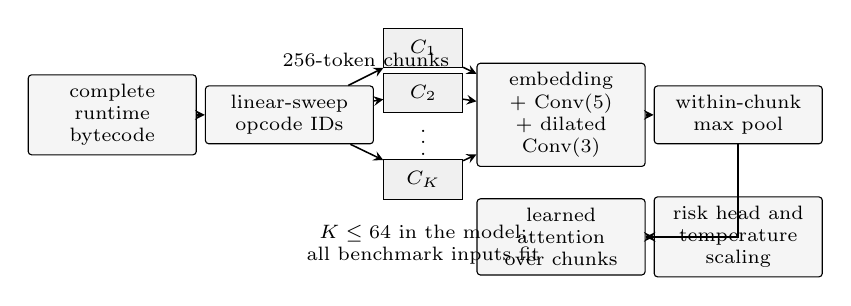
\begin{tikzpicture}[
  font=\scriptsize,
  box/.style={draw, rounded corners=1.2pt, minimum height=7mm, text width=19mm,
              align=center, fill=gray!8},
  small/.style={draw, minimum height=5mm, minimum width=10mm, align=center, fill=gray!12},
  flow/.style={->, >=stealth, line width=.55pt}
]
  \node[box] (bytecode) at (-3.6,0) {complete runtime bytecode};
  \node[box] (tokens) at (-1.35,0) {linear-sweep opcode IDs};
  \node[small] (c1) at (.35,.85) {$C_1$};
  \node[small] (c2) at (.35,.28) {$C_2$};
  \node at (.35,-.25) {$\vdots$};
  \node[small] (ck) at (.35,-.82) {$C_K$};
  \node[box] (local) at (2.10,0) {embedding $+$ Conv(5) $+$ dilated Conv(3)};
  \node[box] (pool) at (4.35,0) {within-chunk max pool};
  \node[box] (attn) at (2.10,-1.55) {learned attention over chunks};
  \node[box] (head) at (4.35,-1.55) {risk head and temperature scaling};
  \draw[flow] (bytecode) -- (tokens);
  \draw[flow] (tokens) -- node[above]{256-token chunks} (c1);
  \draw[flow] (tokens) -- (c2);
  \draw[flow] (tokens) -- (ck);
  \draw[flow] (c1) -- (local);
  \draw[flow] (c2) -- (local);
  \draw[flow] (ck) -- (local);
  \draw[flow] (local) -- (pool);
  \draw[flow] (pool.south) |- (attn.east);
  \draw[flow] (attn) -- (head);
  \node[align=center] at (.35,-1.65) {$K\leq64$ in the model;\\all benchmark inputs fit};
\end{tikzpicture}


  \caption{\model{} preserves local opcode order within 256-token chunks and aggregates evidence
  across the contract. All benchmark programs fit within 64 chunks.}
  \label{fig:encoder}
\end{figure*}

\subsection{Training, calibration, and model selection}

Training minimizes class-weighted binary cross-entropy, with positive weight equal to the
training-fold negative-to-positive ratio. We use AdamW with learning rate $10^{-3}$, weight decay
$10^{-4}$, batch size 16, gradient-norm clipping at 5, a maximum of 30 epochs, and early stopping
after five epochs without validation-AUPRC improvement. Model selection is performed on a
separate validation fold. Temperature scaling then minimizes validation binary cross-entropy on
saved logits, after which warning thresholds are derived only from validation negatives.

We evaluated sequence-only, neural n-gram, dense structural, three-view fusion, multi-task,
source-balanced, and consistency-trained candidates. Table~\ref{tab:model-selection} and
Fig.~\ref{fig:model-selection} show the predeclared validation comparison for seed 7702. The
sequence model led validation AUPRC at 0.9482 and was selected without consulting test AUPRC.
Feature fusion and the auxiliary/consistency objectives are therefore ablations, not causes of
the final result or independent contributions.

\begin{table}[t]
  \centering
  \caption{Validation-led model selection. Values are mean validation AUPRC over five folds for
  seed 7702; test AUPRC was not used for selection.}
  \label{tab:model-selection}
  \scriptsize
  \setlength{\tabcolsep}{3.2pt}
  \begin{tabular}{@{}lr@{}}
    \toprule
    Candidate & Validation AUPRC \\
    \midrule
    \textbf{Hierarchical sequence only} & \textbf{.9482} \\
    Fusion + source-balanced augmentation & .9063 \\
    Fusion + transformation consistency & .8890 \\
    Fusion + multi-task objective & .8644 \\
    Fusion without auxiliary objective & .8568 \\
    Neural hashed n-gram branch only & .8350 \\
    Dense structural branch only & .7051 \\
    \bottomrule
  \end{tabular}
\end{table}



\begin{figure}[t]
  \centering
  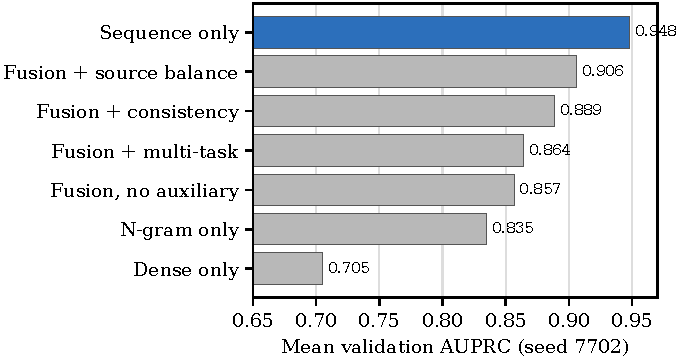
\includegraphics[width=\columnwidth]{figures/validation_model_selection.pdf}
  \caption{Validation-led architecture selection. The sequence-only candidate is highlighted;
  all values precede test-set comparison.}
  \label{fig:model-selection}
\end{figure}

\section{AuthGuardBench-7702}
\label{sec:benchmark}

\subsection{Task-aligned corpus}

The unit of observation is a chain/address pair with associated runtime bytecode. The source
corpus contains four subsets: artifact-derived malicious delegates, contracts not flagged by the
source pipeline (\bclear), broader general contracts (\bgen), and a five-contract verified
account-abstraction control (\baa). The primary task uses the malicious and \bclear{} subsets.
The latter is a weak-negative class: rule silence does not establish benign semantics. The
remaining subsets are controls rather than training positives.

Input alignment was frozen before the current model comparison. Rows containing delegation
designators were resolved to delegate runtime where possible; unresolved designators were
excluded. Complete exact-bytecode groups with conflicting labels were quarantined rather than
retaining a favorable side. The retained benchmark has 3,082 observations and no exact bytecode
shared across primary labels. Same-label redeployments remain because the observational unit is
chain/address; their group membership is made explicit. Table~\ref{tab:dataset} summarizes the
result.

\begin{table}[t]
  \centering
  \caption{AuthGuardBench-7702 composition and dependence controls.}
  \label{tab:dataset}
  \scriptsize
  \setlength{\tabcolsep}{4.0pt}
  \begin{tabular}{@{}lr@{}}
    \toprule
    Item & Count \\
    \midrule
    Malicious primary contracts & 727 \\
    Benign-cleared primary contracts & 1,553 \\
    Primary evaluation population & 2,280 \\
    Benign-general controls & 797 \\
    Benign-AA case observations & 5 \\
    Total observations & 3,082 \\
    Primary bytecode families & 819 \\
    Unique runtime bytecodes & 2,528 \\
    Exact-duplicate groups & 233 \\
    Rows in exact-duplicate groups & 787 \\
    Maximum opcode length & 16,081 \\
    \bottomrule
  \end{tabular}
\end{table}



\subsection{Families and duplicate controls}

The benchmark preserves a pre-existing similarity-family assignment. Runtime bytecode is
linearly disassembled, opcode 4-gram sets are summarized by deterministic 128-permutation BLAKE2b
MinHash signatures, and pairs at the frozen 0.85 signature-agreement threshold are merged by
union--find. The global corpus contains 1,258 families; the primary population contains 819.
Families approximate related code, not attacker identity.

Every primary family is assigned to one of five frozen outer folds. Exact-bytecode groups are
asserted to have one primary label and one primary fold. Thus no training/validation partition
contains members of a held-out test family or exact group. The reduced, task-aligned corpus is not
reclustered or rebalanced after exclusions, which avoids changing dependence definitions in
response to model outcomes.

\subsection{Bounded transformation conditions}

M0 denotes normalized original bytecode. Metadata rewriting modifies a recognized trailer or
adds a synthetic trailer. Address rewriting changes available bytes of selected \code{PUSH20}
immediates. Selector rewriting changes selected sensitive \code{PUSH4} immediates. Flooding
appends \code{STOP} followed by deterministic donor bytes whose amount is a fraction of the
source executable length. F200 uses a factor of 2.0; M3+F200 composes the three rewriting classes
with the flood.

Donor pools are partition-aware. Training, validation, and test transformations draw from
separate family and executable-hash pools so copied bytes do not introduce cross-partition donor
leakage. A ledger records donor provenance. The primary evaluation treats transformed positives
and negatives symmetrically and carries each source label and family into its transformed row.
These transformations test representation sensitivity. They are not labeled new contracts and
do not create independent statistical units.

\subsection{Benchmark artifacts}

\bench{} provides stable sample identifiers, class and provenance fields, bytecode hashes, code
size and opcode count, family and fold assignments, exact-duplicate counts, six observable-factor
fields, a compact opcode-token cache, per-row predictions, validation thresholds, transformation
ledgers, runtime records, and paired-bootstrap summaries. The observable factors document static
surfaces only; they are neither ground-truth vulnerabilities nor auxiliary claims in the selected
model.

\section{Experimental Methodology}
\label{sec:methodology}

\subsection{Family-disjoint protocol}

For outer test fold $f$, fold $(f+1)\bmod 5$ is reserved for validation and the remaining three
folds are used for training. This structure is fixed for every model. Validation selects the
epoch, temperature, and thresholds. Test labels do not influence model selection or policy
construction. We repeat the selected sequence model and strongest baseline with seeds 7702,
7703, and 7704. Results labeled ``three-seed mean'' first average over the five outer folds for
each seed and then average the three seed values.

The paired inferential analysis uses seed 7702 and pools held-out predictions across the five
folds. It draws 10,000 bootstrap samples of primary families with replacement, retains all rows
of each sampled family, and preserves candidate/baseline pairing. This is the correct unit for the
known similarity dependence. Confidence intervals are percentile intervals for the paired
difference. We call a performance gain supported when its interval excludes zero and the direction
is practically favorable.

\subsection{Baselines and ablations}

The strongest evaluated baseline is XGBoost over a 225-dimensional normalized opcode histogram
and a 512-dimensional hashed opcode 4-gram vector. It uses 300 trees, maximum depth 6, learning
rate 0.1, row subsampling 0.9, column subsampling 0.8, and histogram tree construction. It shares
the same training, validation, test rows and validation-negative threshold policy as \model.

Ablations include the neural hashed-4-gram branch, a 261-dimensional dense histogram/structural
branch, their gated fusion with the sequence view, an auxiliary six-factor objective, symmetric
source-balanced transformed training, and a score-consistency penalty. These candidates test
whether modality fusion or transformation-specific training explains performance. They are not
treated as stronger merely because they are more complex.

\subsection{Metrics and operating points}

AUPRC is the threshold-free primary ranking metric because the 31.9\% positive prevalence in the
primary corpus differs from the class ratios expected in deployment. Brier score summarizes
probabilistic error after validation temperature scaling. Operational metrics are recall and
achieved FPR at validation-negative policies targeting 1\%, 5\%, and 10\% FPR. The 5\% policy is
the primary operating point. On \bgen, all rows are controls, so only FPR and Brier score are
defined.

Fold-mean and pooled metrics answer different questions. Three-seed tables describe stability
over training randomization and fold composition. The paired pooled bootstrap estimates the
candidate-baseline difference while respecting family clusters. We do not attach the paired CI
to the three-seed mean, and we do not treat folds or transformed copies as independent samples.

\subsection{Runtime protocol}

Runtime is measured on Linux x86\_64, Python 3.12.12, PyTorch 2.9.0, and CPU inference. A fixed
300-contract sample is scored for ten passes, yielding 3,000 calls with bytecode preloaded. The
timed scope includes sequence preprocessing, model prediction, warning policy, evidence
extraction, and construction of the JSON-ready result. It excludes process startup, model load,
RPC/network access, wallet integration, and UI rendering. Model loading is measured separately.

\section{Evaluation}
\label{sec:evaluation}

We organize results around five research questions. Unless otherwise stated, values are means of
family-disjoint folds and the reported policies are fixed on validation negatives.

\subsection{RQ1: Does the sequence model improve held-out-family detection?}

Table~\ref{tab:three-seed} gives the descriptive three-seed results. On clean M0, \model{} obtains
0.9309 AUPRC compared with 0.8276 for histogram+n-gram XGBoost, an absolute difference of 0.1033
in the descriptive means. Recall at the 5\% policy is 0.8282 versus 0.5822, while achieved FPR is
0.0463 versus 0.0631. The sequence model also has lower Brier error, 0.0622 versus 0.1392. The
direction holds for each of the three seeds; its seed-level clean AUPRC SD is 0.0090.

At the stricter 1\% policy, \model{} recalls 0.6008 of positive rows, compared with 0.3396 for the
baseline. At the 10\% policy, the corresponding recalls are 0.9297 and 0.7078. These points show
that the improvement is not confined to one threshold, although achieved FPR can differ from the
nominal validation budget.

\begin{table*}[t]
  \centering
  \caption{Family-disjoint performance. Each entry is the mean over five folds and three training
  seeds; parenthesized values are population SDs across the three seed-level fold means. Policies
  are fitted using validation negatives.}
  \label{tab:three-seed}
  \scriptsize
  \setlength{\tabcolsep}{4.2pt}
  \begin{tabular}{@{}llcccccc@{}}
    \toprule
    Condition & Model & AUPRC & Recall@1 & Recall@5 & Recall@10 & FPR@5 & Brier \\
    \midrule
    Clean M0 & AuthGuard-Seq & \textbf{.9309} (.0090) & \textbf{.6008} & \textbf{.8282} & \textbf{.9297} & \textbf{.0463} & \textbf{.0622} \\
             & Hist.+4-gram XGB & .8276 (.0111) & .3396 & .5822 & .7078 & .0631 & .1392 \\
    \midrule
    F200 & AuthGuard-Seq & \textbf{.9104} (.0070) & \textbf{.2928} & \textbf{.7235} & \textbf{.8439} & \textbf{.0315} & \textbf{.0930} \\
         & Hist.+4-gram XGB & .5765 (.0062) & .0427 & .1714 & .2922 & .0446 & .2581 \\
    \midrule
    M3+F200 & AuthGuard-Seq & \textbf{.9102} (.0137) & \textbf{.2951} & \textbf{.7189} & \textbf{.8544} & \textbf{.0407} & \textbf{.0941} \\
            & Hist.+4-gram XGB & .5633 (.0141) & .0331 & .1788 & .2947 & .0421 & .2587 \\
    \bottomrule
  \end{tabular}
  \vspace{1pt}

  \parbox{.96\textwidth}{\scriptsize Recall@$q$ and FPR@$q$ use the threshold selected at nominal
  $q\%$ validation-negative FPR. They are not thresholds selected on the test set.}
\end{table*}



Table~\ref{tab:bootstrap} gives the separate paired analysis. Pooled clean AUPRC is 0.8910 for
\model{} and 0.8339 for the baseline. The paired delta is $+0.0571$ with 95\% CI
$[+0.0023,+0.1179]$. Recall@5 improves by $+0.2118$ with CI
$[+0.0952,+0.3390]$, and achieved FPR decreases by 0.0245. Therefore the evidence supports the
bounded claim that the sequence model outperforms the strongest evaluated bytecode baseline on
clean \bench{} held-out families. It does not support superiority over systems trained for other
labels or over unbenchmarked static analyzers.

\begin{table*}[t]
  \centering
  \caption{Primary-seed paired family-clustered comparison against the strongest baseline. Values
  pool held-out rows across five folds; CIs use 10,000 paired family-bootstrap replicates.}
  \label{tab:bootstrap}
  \scriptsize
  \setlength{\tabcolsep}{4.2pt}
  \begin{tabular}{@{}llrrrrl@{}}
    \toprule
    Condition & Metric & Sequence & Baseline & $\Delta$ & \multicolumn{1}{c}{95\% CI for $\Delta$} \\
    \midrule
    Clean M0 & AUPRC & .8910 & .8339 & +.0571 & $[+.0023,+.1179]$ \\
             & Recall@5 & .8391 & .6272 & +.2118 & $[+.0952,+.3390]$ \\
             & achieved FPR@5 & .0341 & .0586 & -.0245 & $[-.0466,-.0047]$ \\
    \midrule
    F200 & AUPRC & .8828 & .5513 & +.3314 & $[+.2561,+.4089]$ \\
         & Recall@5 & .7538 & .1733 & +.5805 & $[+.4678,+.6794]$ \\
         & achieved FPR@5 & .0212 & .0438 & -.0225 & $[-.0372,-.0090]$ \\
    \midrule
    M3+F200 & AUPRC & .8693 & .5439 & +.3254 & $[+.2561,+.4016]$ \\
            & Recall@5 & .7552 & .2091 & +.5461 & $[+.4365,+.6435]$ \\
            & achieved FPR@5 & .0354 & .0361 & -.0006 & $[-.0166,+.0143]$ \\
    \bottomrule
  \end{tabular}
\end{table*}



\subsection{RQ2: Which architectural choice accounts for performance?}

The validation comparison in Table~\ref{tab:model-selection} rejects the originally hypothesized
multi-view explanation. Sequence-only validation AUPRC is 0.9482. Adding hashed n-grams and dense
features without auxiliary supervision yields 0.8568; the multi-task candidate reaches 0.8644;
source-balanced transformation training reaches 0.9063; and the consistency candidate reaches
0.8890. None surpasses the selected model.

The primary-seed clean test ablation is consistent with selection: fold-mean AUPRC is 0.9182 for
the sequence model, 0.8411 for histogram+n-gram XGBoost, 0.8331 for consistency-trained fusion,
0.8145 for source-balanced fusion, 0.8078 for multi-task fusion, 0.7936 for fusion without
auxiliary tasks, 0.7874 for the neural n-gram view, and 0.6377 for the dense view. Under F200, the
sequence result remains 0.9006, compared with 0.7062--0.7251 for the strongest fusion training
variants. Complexity alone did not improve the task.

We infer that ordered local patterns combined with contract-wide aggregation are the useful
inductive bias in this corpus. This is an empirical explanation, not proof that n-grams or
structural features are generally unhelpful. The negative result narrows the paper's architecture
claim and avoids attributing gains to auxiliary tasks that the selected artifact does not use.

\subsection{RQ3: How does performance change under bounded transformations?}

Figure~\ref{fig:robustness} and Table~\ref{tab:three-seed} compare clean, F200, and M3+F200
conditions. \model{} changes from 0.9309 clean AUPRC to 0.9104 under F200 and 0.9102 under
M3+F200. The baseline falls from 0.8276 to 0.5765 and 0.5633. Recall@5 for \model{} is 0.7235 and
0.7189 in the transformed arms, compared with 0.1714 and 0.1788 for XGBoost. Thus the selected
sequence model degrades modestly under the defined stressors while the baseline's ranking and
low-FPR recall degrade sharply.

\begin{figure*}[t]
  \centering
  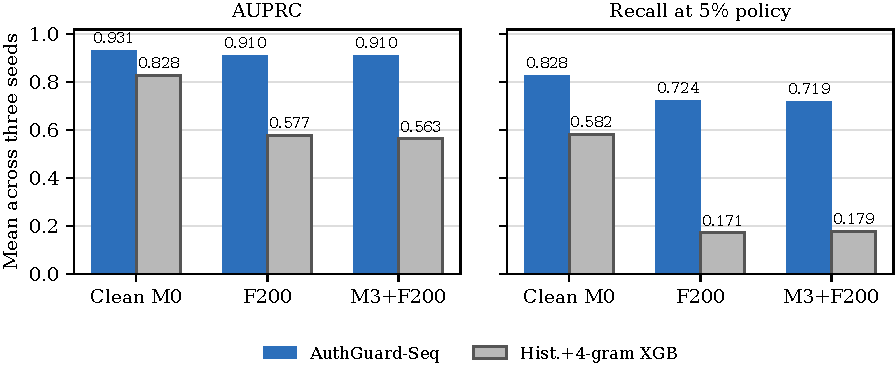
\includegraphics[width=.88\textwidth]{figures/clean_and_transformed_performance.pdf}
  \caption{Three-seed family-disjoint performance under clean and bounded transformed
  conditions. F200 is donor-isolated 200\% post-\code{STOP} flooding; M3+F200 additionally applies
  metadata, address, and selector rewriting.}
  \label{fig:robustness}
\end{figure*}

The paired estimates are larger under transformation. For F200, the AUPRC delta is $+0.3314$
with CI $[+0.2561,+0.4089]$ and Recall@5 improves by $+0.5805$. For M3+F200, AUPRC improves by
$+0.3254$ and Recall@5 by $+0.5461$, with both intervals excluding zero. The F200 achieved-FPR
difference favors \model, whereas the M3+F200 FPR difference is unresolved
($-0.0006$, CI $[-0.0166,+0.0143]$). We therefore claim higher ranking and recall under these
protocol transformations, not uniformly lower FPR and not universal adversarial robustness.

The results also illustrate why a representation audit matters. A first-\code{STOP}
representation reached approximately 0.970 AUPRC in a separate diagnostic and appeared invariant
to these transformations, but 92/100 bounded calls executed code after the first linear-sweep
\code{STOP}; truncation preserved the execution fingerprint in only 22/100. We exclude that
representation from \model{} and retain the finding as a warning that predictive shortcuts can
look robust precisely because the stressor modifies discarded bytes.

\subsection{RQ4: What false-alert tradeoff remains?}

On \bgen, \model's three-seed mean FPRs are 0.0051, 0.0616, and 0.1000 at the 1\%, 5\%, and 10\%
policies. The baseline's corresponding values are 0.0086, 0.0452, and 0.0727. At the primary 5\%
policy, the sequence model therefore raises more benign-general alerts in the descriptive mean.
In the primary-seed pooled analysis, the FPRs are 0.0853 and 0.0376; the paired difference is
$+0.0477$ with CI $[-0.0202,+0.1501]$, which does not exclude zero.

These observations prohibit a claim that \model{} reduces benign-general false alerts. The
primary population and broader benign controls differ in source and family composition, so a
threshold calibrated on primary validation negatives need not transfer exactly. A practical
integration should make the policy configurable, monitor alert prevalence after deployment, and
recalibrate on a representative benign population. The 1\% tier offers a stricter default when
warning fatigue is costly; the 5\% and 10\% tiers can support escalation or analyst review rather
than blocking.

\begin{table}[t]
  \centering
  \caption{Operational controls for AuthGuard-Seq. Benign-control FPRs are three-seed means;
  runtime is over 3,000 local CPU calls.}
  \label{tab:operational}
  \scriptsize
  \setlength{\tabcolsep}{3.0pt}
  \begin{tabular}{@{}lr@{}}
    \toprule
    Measurement & Value \\
    \midrule
    benign-general FPR@1 & .0051 \\
    benign-general FPR@5 & .0616 \\
    benign-general FPR@10 & .1000 \\
    \midrule
    Model artifact & 742,561 bytes \\
    Model load & 10.047 ms \\
    Mean local screening & 4.334 ms \\
    Median local screening & 3.172 ms \\
    p95 local screening & 14.073 ms \\
    p99 local screening & 16.906 ms \\
    \bottomrule
  \end{tabular}
\end{table}



\subsection{RQ5: Is local screening operationally lightweight?}

The selected artifact occupies 742,561 bytes (approximately 0.743 MB). Over 3,000 CPU calls, mean
local screening time is 4.334 ms, median 3.172 ms, p95 14.073 ms, and p99 16.906 ms. Loading the
model once takes 10.047 ms in the measured environment. The worst observed local call is 21.066
ms. These values support the claim that the scorer itself is lightweight enough to be considered
for an interactive integration.

They do not establish end-to-end wallet latency. RPC lookup, network variability, process
startup, proxy resolution, wallet rendering, and user interaction are explicitly excluded. A
persistent integration can amortize model loading, whereas a one-shot CLI invocation will incur
additional startup overhead. The appropriate statement is therefore ``4.334 ms mean local
screening latency in the measured environment,'' not ``sub-5 ms authorization'' or a guaranteed
latency bound.

\section{Discussion}
\label{sec:discussion}

\subsection{Why a hierarchical sequence view is useful}

Opcode histograms discard order, and hashed 4-grams retain only short local context. Their
combination is strong on clean bytecode but is sensitive to large amounts of donor padding. The
hierarchical model preserves local ordered patterns through convolution, compresses each chunk,
and learns which chunks contribute to the contract representation. Because attention normalizes
over chunks, flooding can still influence the representation, but appended material does not
simply dominate a global count vector. This mechanism is consistent with the observed robustness
gap, although the experiments do not isolate attention normalization as a causal factor.

Long-input coverage is also important. A fixed 1,024- or 4,096-token prefix would omit substantial
portions of several contracts. The 16,384-token capacity covers every benchmark program and the
even-spacing fallback avoids a pure prefix for larger inputs. The first-\code{STOP} audit further
shows that seemingly principled truncation can be invalid in the EVM, where dispatcher paths can
jump to later \code{JUMPDEST} blocks. Full-stream coverage is therefore both an architectural
choice and a safeguard against one identified shortcut.

\subsection{Role in a defense stack}

\system{} is best interpreted as a triage layer. A wallet or security service can score a proposed
delegate locally, display the directly observed surfaces, and invoke decompilation, symbolic
analysis, simulation, reputation, or human review for elevated tiers. The scorer can also be used
by registries and monitoring systems before newly observed delegates accumulate behavior. This
positioning avoids a false choice between fast ML and semantic analysis: their information and
cost profiles are complementary.

The structured interface is necessary but not sufficient for useful deployment. A real wallet
must bind the displayed result to the exact chain, address, block, and authorization being signed;
resolve delegation and proxy indirection; protect model and threshold provenance; and explain
that low observed risk is not approval. The four-tier policy supports this communication better
than a binary safety label, but user studies are required to validate warning comprehension.

\subsection{Lessons from unsuccessful alternatives}

Three negative findings improve the final design. First, feature fusion and auxiliary factor
prediction did not beat the sequence-only model, so direct observable evidence is kept outside
the risk head. Second, transformation-consistent and source-balanced training did not establish a
separate learning contribution; the unaugmented sequence model generalized better in validation.
Third, first-\code{STOP} produced excellent predictions but failed semantic scrutiny. These
results argue for validation-led simplification and for auditing unusually strong representations
before turning them into a novelty claim.

Adaptive random and beam searches remain useful stress-test tooling, but search itself is not the
paper's contribution. Their bounded execution checks also expose a key distinction: an action can
reduce a model score while changing execution. Robustness evaluation should therefore report both
classifier outcomes and preservation evidence, rather than assuming that byte-level edits are
behavior-neutral.

\section{Limitations and Responsible Use}
\label{sec:limitations}

\textbf{Label scope.} Positive labels originate from one EIP-7702 security artifact, while
\bclear{} denotes absence of that pipeline's finding rather than verified benign behavior. The
model may learn properties of source collection or rule coverage. Family grouping, task
alignment, and duplicate controls reduce leakage but do not make the labels complete or
independent. Results should be phrased as delegate-risk screening on this task, not universal
vulnerability detection.

\textbf{External and temporal validity.} The benchmark does not provide a defensible temporal
field, so no temporal holdout is synthesized from row order. Chain and family controls cannot
predict performance on future compiler patterns, newly popular delegate frameworks, or new
attacks. Independent, time-indexed EIP-7702 corpora are needed for stronger generalization claims.

\textbf{Benign coverage.} The 797 \bgen{} controls broaden negative evaluation, but the five
\baa{} observations are qualitative cases, not a statistical estimate of account-abstraction
compatibility. The observed 5\% benign-general false-alert rate is an operational concern.
Calibration and thresholds must be revisited for each deployment population.

\textbf{Static information.} Runtime bytecode alone omits storage state, proxy targets, calldata,
counterparties, signer assets and approvals, transaction ordering, and off-chain intent. Direct
opcode observations are not reachable-path proofs. A benign-looking implementation can become
dangerous through state or indirection, and a high-risk surface can be safely constrained by
logic the model does not understand.

\textbf{Transformation validity.} F200 has strong bounded execution preservation on the ten
audited contracts, but this sample is small. Address and selector rewrites often change the raw
execution fingerprint and are not preservation-oriented. M3+F200 results quantify representation
stress, not semantic adversarial accuracy. Arbitrary recompilation, control-flow rewriting, and
white-box attacks remain open.

\textbf{Operational completeness.} The tool is integration-ready but not deployed. We do not
measure network or end-to-end wallet latency, proxy-resolution accuracy, human warning response,
or production model-update security. The software should not automatically approve
authorizations or be presented as a safety certificate.

\textbf{Responsible release.} Per-row benchmark and transformation artifacts can support
reproduction and defense research. Any release should retain provenance, transformation scope,
and residual-risk notices. Evaluation code should preserve family/duplicate constraints so that
convenient random splits do not become the reported result.

\section{Conclusion}
\label{sec:conclusion}

We presented \system, a bytecode-only pre-authorization screener for EIP-7702 delegate contracts;
\model, its hierarchical full-bytecode opcode-sequence architecture; and \bench, a
dependence-aware evaluation framework. Across three seeds, the selected model achieves 0.931
clean AUPRC and approximately 0.910 AUPRC under F200 and M3+F200, outperforming the strongest
evaluated histogram+n-gram baseline in paired family-clustered comparisons. A 0.743 MB artifact
performs local preprocessing, inference, policy evaluation, and evidence construction in 4.334
ms on average in the measured CPU environment. These findings support lightweight screening at
the authorization boundary, while source-derived labels, benign-control false alerts, bounded
transformation validity, and unevaluated wallet integration set clear limits. The resulting
system is a practical first-stage risk signal, not a proof that delegated code is safe.

\appendices

\section{Reproducibility Details}
\label{app:reproducibility}

Table~\ref{tab:hyperparameters} records the principal model and baseline settings. All candidates
share the same frozen outer folds and validation rotation. The implementation records per-row
scores, family identifiers, model, condition, seed, and fold; threshold files and model artifacts
record calibration and policy values. The primary paired analysis is reproducible from held-out
prediction rows without retraining.

\begin{table}[h]
  \centering
  \caption{Principal training and representation settings.}
  \label{tab:hyperparameters}
  \scriptsize
  \setlength{\tabcolsep}{3.0pt}
  \begin{tabular}{@{}lr@{}}
    \toprule
    Setting & Value \\
    \midrule
    Outer folds & 5 family-disjoint \\
    Training seeds & 7702, 7703, 7704 \\
    Chunk width / maximum chunks & 256 / 64 \\
    Opcode embedding & 32 \\
    Convolution channels & 64 \\
    Convolution kernels & 5; 3 (dilation 2) \\
    Risk representation & 128 \\
    Dropout & .15 \\
    Optimizer / learning rate & AdamW / $10^{-3}$ \\
    Weight decay / batch size & $10^{-4}$ / 16 \\
    Maximum epochs / patience & 30 / 5 \\
    XGBoost trees / depth & 300 / 6 \\
    Bootstrap replicates & 10,000 \\
    \bottomrule
  \end{tabular}
\end{table}

\section{Complete Operating-Point Summary}
\label{app:operating}

Table~\ref{tab:operating-full} reports achieved FPRs corresponding to the recalls in
Table~\ref{tab:three-seed}. Policies are estimated independently in each seed/fold validation
partition. Consequently, achieved held-out FPR can exceed the nominal level, especially under
population or transformation shift.

\begin{table*}[h]
  \centering
  \caption{Three-seed mean recall and achieved FPR at all validation-matched policies.}
  \label{tab:operating-full}
  \scriptsize
  \setlength{\tabcolsep}{4.2pt}
  \begin{tabular}{@{}llrrrrrr@{}}
    \toprule
    Condition & Model & Recall@1 & FPR@1 & Recall@5 & FPR@5 & Recall@10 & FPR@10 \\
    \midrule
    Clean M0 & AuthGuard-Seq & .6008 & .0164 & .8282 & .0463 & .9297 & .0955 \\
             & Hist.+4-gram XGB & .3396 & .0194 & .5822 & .0631 & .7078 & .1196 \\
    F200 & AuthGuard-Seq & .2928 & .0059 & .7235 & .0315 & .8439 & .0604 \\
         & Hist.+4-gram XGB & .0427 & .0061 & .1714 & .0446 & .2922 & .0899 \\
    M3+F200 & AuthGuard-Seq & .2951 & .0047 & .7189 & .0407 & .8544 & .0797 \\
            & Hist.+4-gram XGB & .0331 & .0060 & .1788 & .0421 & .2947 & .0925 \\
    \bottomrule
  \end{tabular}
\end{table*}

\section{Tool Output Contract}
\label{app:tool}

The following abbreviated schema illustrates fields returned by the selected sequence artifact.
Values shown are types or placeholders, not one evaluated contract. Only deterministic observed
evidence is used as explanatory content.

\begin{lstlisting}[language={}]
{
  "schema_version": "authguard-7702-score-v1",
  "target": "0x...",
  "bytecode_sha256": "...",
  "risk_score": 0.0,
  "warning_level": "high|warning|caution|low_observed_risk",
  "warning_policy": {"fpr_01": 0.0, "fpr_05": 0.0, "fpr_10": 0.0},
  "observed_evidence": {
    "code_bytes": 0,
    "opcode_count": 0,
    "opcode_counts": {"CALL": 0, "DELEGATECALL": 0, "SSTORE": 0},
    "token_movement_selectors": [],
    "approval_selector": null,
    "observed_factors": {}
  },
  "top_opcode_chunks": [0],
  "local_scorer_ms": 0.0,
  "scope_notice": "A low score is not a safety guarantee..."
}
\end{lstlisting}

\section{Negative Results and Claim Decisions}
\label{app:negative}

The extended study evaluated several plausible but unsupported contribution paths:
\begin{itemize}
  \item \textbf{Multi-view and multi-task learning.} Neither gated fusion nor the observable-factor
  auxiliary task surpassed sequence-only validation AUPRC. The selected tool therefore reports
  direct observations rather than auxiliary predictions.
  \item \textbf{Transformation-consistent training.} Symmetric transformation training and a
  score-consistency penalty improved some fusion stress-test results but remained below the
  unaugmented sequence model. The procedure is an ablation, not a separate contribution.
  \item \textbf{First-\code{STOP} representation.} Its high AUPRC did not correspond to an
  executable prefix: post-\code{STOP} code was commonly reachable and executed. It is retained
  only as a warning about predictive shortcuts.
  \item \textbf{Conservative canonicalization.} The reachability-aware extractor passed a bounded
  execution check but failed the predefined predictive non-inferiority criterion relative to full
  bytecode. It is not part of the proposed system.
  \item \textbf{Adaptive search.} Random and beam searches provide stress cases and query-cost
  evidence, but search is neither the final architecture nor a standalone paper contribution.
\end{itemize}

These decisions are scientifically material because they distinguish the system that the
evidence selects from the more elaborate system originally hypothesized.

\bibliographystyle{IEEEtran}
\bibliography{references}

\end{document}
